\documentclass[11pt]{article}
\usepackage[a4paper margin=3cm]{geometry}
\usepackage{hyperref}
\usepackage{amsmath}
\usepackage{svg}
\usepackage{textcomp}
\usepackage{gensymb}
\usepackage{enumitem}
\usepackage{listings}
\usepackage{booktabs}
\usepackage{subcaption}
\usepackage{calc}
\usepackage{todonotes}

\begin{document}

\title{Coherent and Colorful Image Colorization}
\author{Florian Stellbrink\\\texttt{\href{mailto:gusstefl@student.gu.se}{gusstefl@student.gu.se}}}
\maketitle

\section{Introduction}
Looking at the grayscale picture in \autoref{fig:example} we intuitively understand that the sky is at the top and grass covers most of the ground. Using this knowledge we can color the image with blue and green colors.
Zhang~et~al.~\cite{zhang2016colorful} propose a method to teach this understanding and the ability to colorize images to machines. 

We present a new model that extends the approach of Zhang~et~al.~\cite{zhang2016colorful}. It is going to directly use contextual information which has not been used by the original authors to achieve coherence. Using a definition of spatial coherence that does not rely on specific colors enables us to select colors from distributions without compromising color saturation.

Zhang~et~al.~\cite{zhang2016colorful} point out that grayscale pixels may correspond to different colors. A ball for example might be blue or red, even though its brightness does not change. By minimizing the error in every training step, these algorithms converge on an average of all possible colors. Unfortunately the average of multiple possible colors can be implausible. Estimating brown as the average of blue and red may minimize the error function, but is unlikely to convince a human who was expecting a colorful object.
Instead, their approach involves a probability distribution over all possible colors. That allows the network to predict colorful but rare colors.

Understanding this new approach requires an understanding of the previous approaches. The next sections will explain the key steps and their relevance to the goal of colorful colorizations. Afterwards, we are going to present the idea and implementation of the new approach and look at the results.

\section{Fundamentals}

The same grayscale value can belong to different colors, even when it occurs in the same context. Zhang~et~al.\cite{zhang2016colorful} expressed this property in their model and preserved color in three steps:

\begin{itemize}
    \item Instead of predicting a single color, they estimate the probabilities of different colors. This prevents the averaging effects of previous approaches.
    \item Colors in images are inherently imbalanced. Unsaturated colors are more common leading to an unbalanced dataset. We will have a look at the rebalancing term that compensates for this imbalance in \autoref{chap:rebalancing}.
    \item The final step of the original paper translates color distributions into colors. This is what we attempt to improve and key to understanding the new approach.
\end{itemize}

The original authors determined the quality of their results in a study with human subjects. The subjects get to see a pair of colored images and have to decide which one is the ground truth and which one has been colorized. Ideally the two images are indistinguishable and results are blind guesses, in this case both images would have a $50\%$ chance of being chosen. The participants of this study deemed the re-colorized image to be the original $32\%$ of the time. 

\begin{figure}
    \includesvg[width=\textwidth]{latex/example}
    \caption{
    Example of image colorization. The first row shows original, grayscale, and recolorized images for both colorful outputs from Zhang~et~al~\cite{zhang2016colorful} and our coherent result.
    The second row shows the same examples with the grayscale component set to a uniform value of $L=50$. This shows the differences in the color channels more clearly.
    }
    \label{fig:example}
\end{figure}

\subsection{Classification}
\label{chap:classification}
when predicting colors simple regression from grayscale to color values will have an averaging effect. Since we want to find vibrant and convincing colors, we are instead going to predict probabilities for individual colors.

To do that we have to find a finite set of colors which we can represent as a vector of probabilities. During training the network will learn to assign higher probabilities to colors it encounters, but it will never have to average these likely values.

\subsubsection*{Color Space}
For classification we need to find a discrete set of colors. To select them we use the CIELab color space which consists of three channels:
\begin{itemize}
    \item $L$: For the luminance or brightness.
    \item $a$: For the color's blue-yellow component.
    \item $b$: For the red-green component.
\end{itemize}
Only values for $a$ and $b$ need to be estimated, since we use the grayscale brightness as a value for $L$ directly. We choose classes by sampling this color space every $10$ units on the $a$ and $b$ axis while setting $L$ to $50$. The color palette chosen by Zhang~et~al.~\cite{zhang2016colorful} is shown in \autoref{fig:lab}a.

\begin{figure}[tbp]
    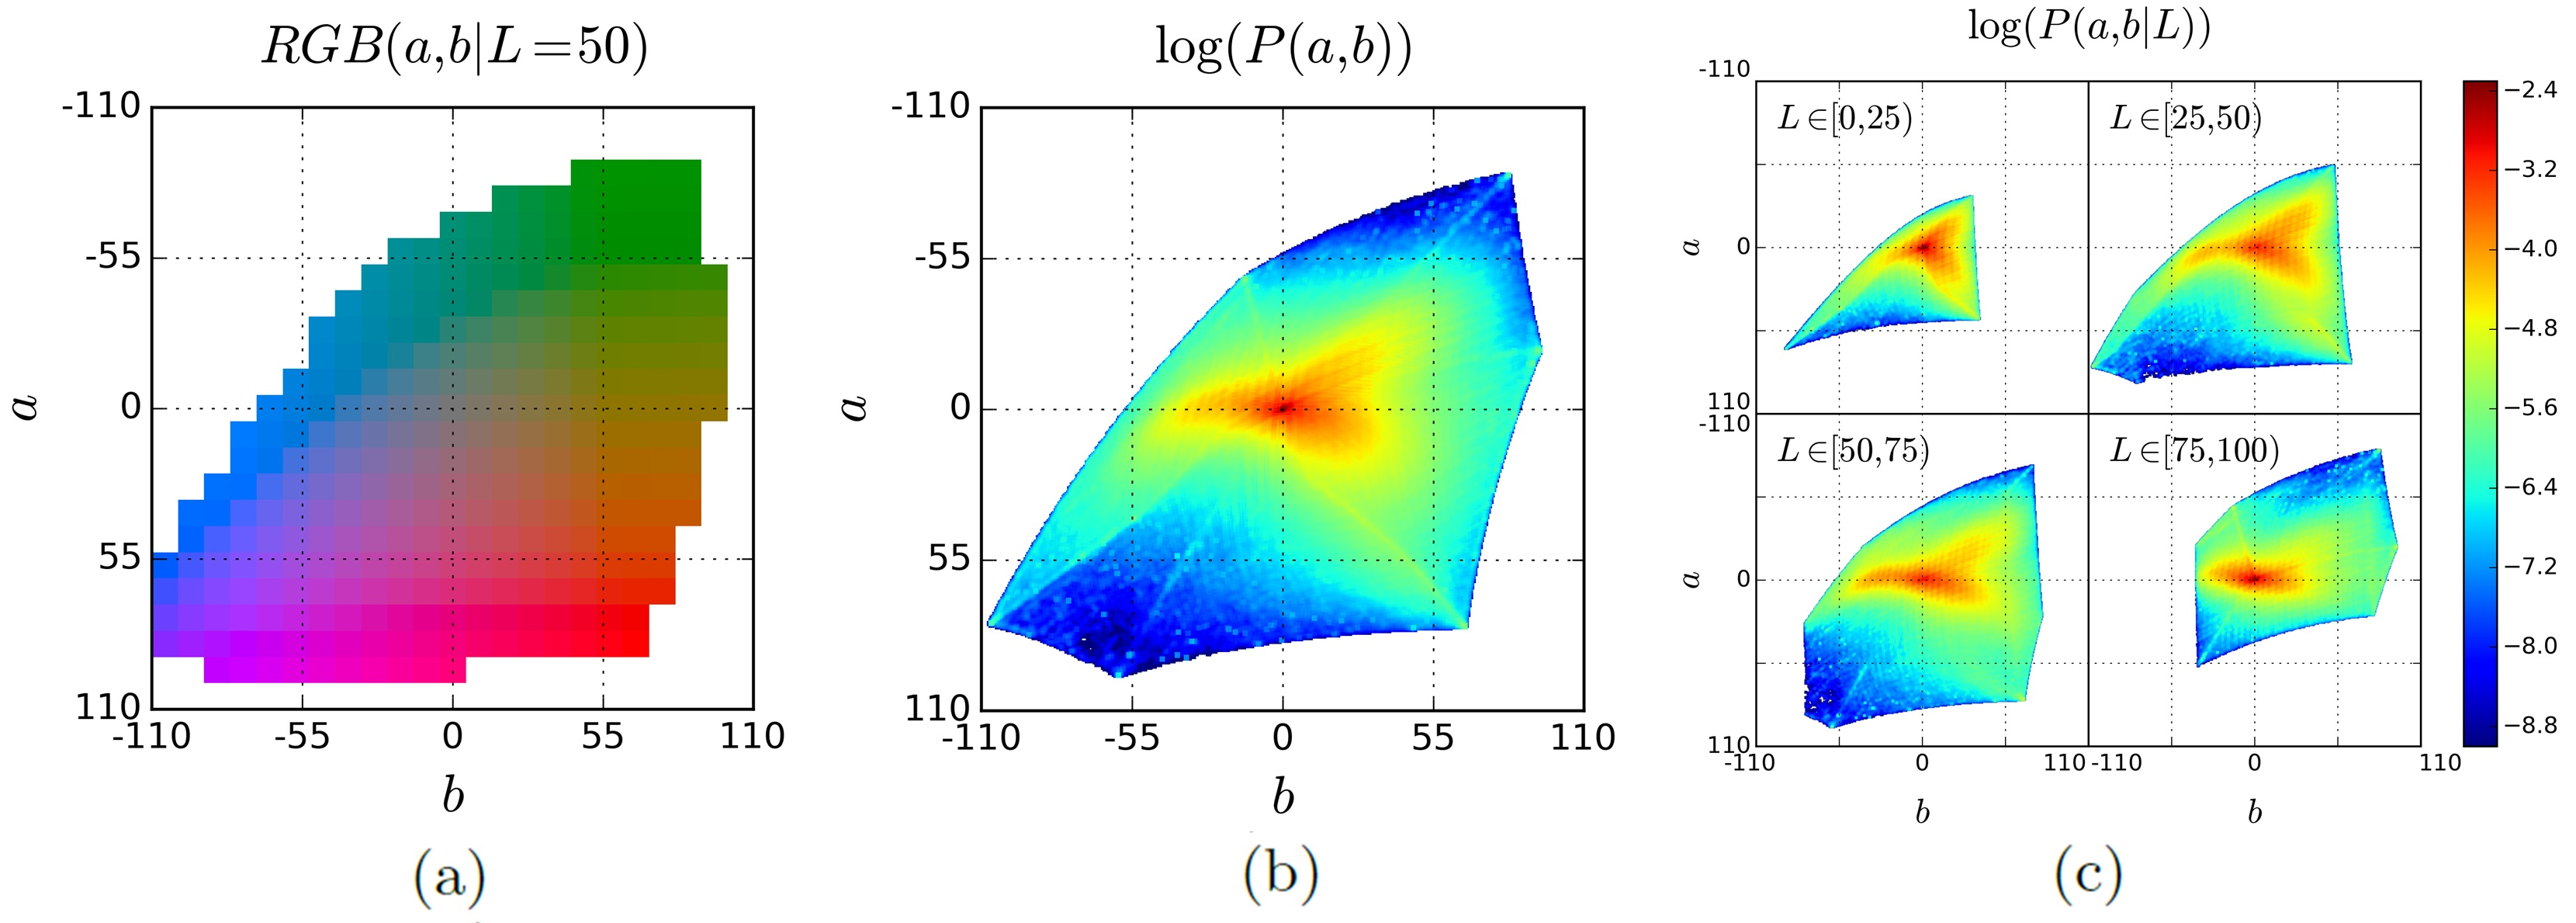
\includegraphics[width=\textwidth]{latex/lab.jpg}
    \caption{CIELab color space visualization from \cite{zhang2016colorful}. (a) Shows all colors used for classification. (b) Depicts color frequencies within the training set. (c) Shows how those frequencies change with luminance.}
    \label{fig:lab}
\end{figure}

\subsection{Rebalancing}
\label{chap:rebalancing}
We want the network to understand the context of pixels within images and feed it entire images to achieve that. Unfortunately colors are usually not equally distributed in photographs or other images. In fact some colors are more common than others by orders of magnitude. \autoref{fig:lab} shows the frequencies at which colors occur in the training set chosen by Zhang~et~al\cite{zhang2016colorful}. As you can see desaturated colors are most frequent and will dominate the training. Because the training facility is rewarded for picking them, it will learn to predict desaturated colors.

To compensate for that we use weights for every pixel in our objective function. This weight will compensate the uneven distribution of colors by weighing rare colors more than common colors. To find these weights we first need to find the empirical distribution of colors in the training set $p$. If we chose this as a weight we would get very high probabilities for very unlikely but rare colors. Instead we mix that distribution with the normal distribution $\frac{1}{Q}$ where $Q$ is the size of our color palette.

\begin{align}
    w \propto \left(\left( 1-\lambda \right) p + \frac{\lambda}{Q} \right)^{-1}
\end{align}

We set $\lambda=\frac{1}{2}$ to get a decent trade off between influence of rare colors and common colors.

\subsection{Color Selection}
\label{chap:selection}
While color classes are useful for training we ultimately want to output a single color for each pixel. Two ways of doing that are choosing the class with the highest probability, i.e. the distribution's mode, or its average. While choosing the most probable value results in vibrant colors it lacks spatial coherence, i.e. pixels in the same image region can have very different colors. Choosing the mean instead leads to a coherent result, but now the colors look desaturated.  

Instead of choosing either of those options the authors use a function that seamlessly interpolates between both of them and chose a parameter that produces a convincing middle ground. This function is a modification of the softmax function that adds an additional temperature parameter $T$:

\begin{align} \label{eq:softmax}
    f_T(z) = \frac{exp(log(z)/T)}{\sum_q{exp(log(z_q)/T)}}
\end{align}

The idea with this function is that $exp$ and $log$ lead to a function that behaves similar to $log$ by itself when $T=1$. But when $T \rightarrow 0$ it changes to exponential behaviour where larger values will dominate smaller values, turning softmax into a one-hot encoding in the limit.

When we pick the mean of a distribution after applying this function to it, we can interpolate between picking the mean of the original distribution and its mode, by changing $T$. This is true since the mean of the one hot encoding we get for $T \rightarrow 0$ is the original distribution's mode.

Zhang~et~al\cite{zhang2016colorful} chose a value of $T=0.38$, which they considered a good trade off between saturation and spatial coherence.

\begin{figure}
    \includesvg[width=\textwidth]{output/example0-1}
    \caption{
    Example of color bleeding. Even though the ceiling is a single uniform surface, blue start to show up within.
    }
    \label{fig:example-bleed}
\end{figure}

\section{Coherence from Context}

When we consider the method for color selection we just presented, we are going to notice that it only involves a single pixel's color distribution. This immediately discards any contextual information that might have been used for spatially coherent colors. Zhang~et~al\cite{zhang2016colorful} explain that choosing the mean of a distribution leads to some spatial coherence, but there are limitations to that approach. When looking at \autoref{fig:example-bleed} we can see that colors sometimes bleed into areas, they are not supposed to and that sometimes colors change within the same surface. This is immediately obvious to humans, because we can recognize surfaces and usually do not expect colors to extend beyond them or suddenly change within them. We even have those expectations when we see grayscale images, which gives away what images are re colorized in those instances.

Now the idea is to replace the previous selection of colors with a new neural network, which is depicted in \autoref{fig:architecture}. That network is supposed to transform the predicted distribution of colors in a way that makes the mode of that distribution spatially coherent. There are two details we have to get right to teach this to our network:

\begin{enumerate}
    \item We cannot use specific colors in the objective function. That would turn the entire method into a regression system and discard any advantage we had gotten from using distribution in the first place.
    \item We need to stay as true as possible to the original distribution. More specifically, the mode of the new distribution needs to be as likely as possible in the original distribution. If it weren't we would end up with a distribution that is spatially coherent, but makes no use of the previously predicted colors.
\end{enumerate}

When we achieve those goals, we expect to arrive at color predictions that are vibrant while not suffering from spatial incoherence. The next two sections will walk through the ideas behind both points, their definitions, and their implementation.

\begin{figure}[tbp]
    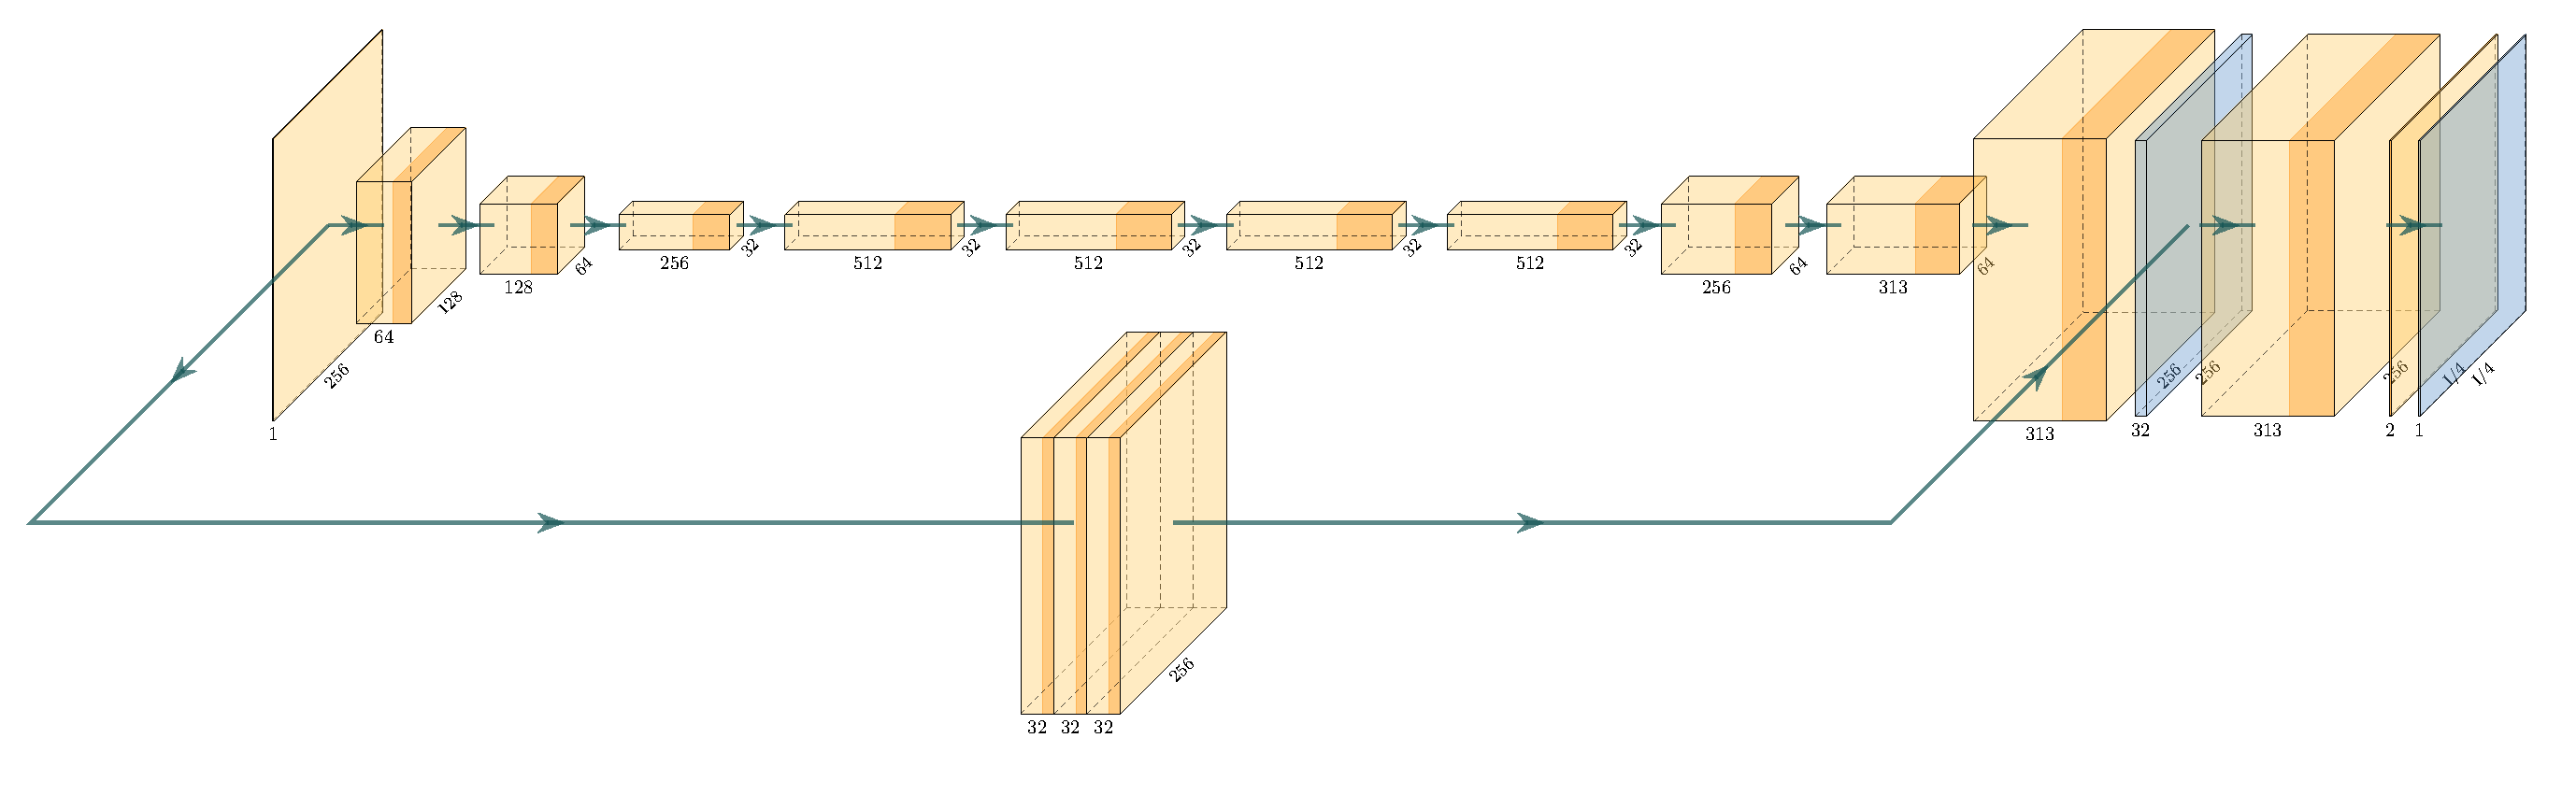
\includegraphics[width=\textwidth]{latex/architecture.pdf}
    \caption{Model architecture visualization. The model starts similar to  Zhang~et~al.\cite{zhang2016colorful} on the top track. A separate branch runs convolution on the grayscale input and is concatenated with the up-scaled color distributions. Finally distributions and CIELab colors are predicted from the concatenation of both branches, with the luminance component being taken straight from the input.}
    \label{fig:architecture}
\end{figure}

\subsection{Spatial Coherence}
\label{chap:coherence}

When we talk about spatial coherence, we can define it as the absence of color bleeding and sudden color changes within surfaces. Unfortunately, this informal definition is not going to be useful for the implementation.

It is going to be hard to define coherence by only using the predicted image. Instead, we are going to define it as a function of both the ground truth image and the predicted image. We are going to assume that the ground truth images adhere to our informal definition of coherence, so we can use them as a frame of reference.

As stated before we cannot compare the predicted image directly to the ground truth, since that would yield a regressive prediction. In place of a direct comparison we are going to compare the gradients of both images. A gradient in the context of two dimensional images is the change of a color in both horizontal or vertical direction within either of the two color channels $a$ and $b$.

The color channels are $a$ and $b$, since we are still working in the CIELab color space. This has two big advantages over RGB:
\begin{itemize}
    \item It allows us to ignore the luminance, which we are not predicting anyway.
    \item Euclidean distances within this space are similar to the perceived distance of those colors, thanks to perceptional uniformity \cite{paschos2001perceptually,johnson2016perceptual}.
\end{itemize}

The distance between both gradients in that space is defined by $L_C$, give the ground truth $Y$ and prediction $\hat{Y}$:

\begin{align}
    L_C(\hat{Y}, Y) = \sum_{h, w}{\left\lVert \Delta Y_{h,w} - \Delta \hat{Y}_{h,w}\right\rVert_2}
\end{align}

This metric makes sure that a change in color of the original image encourages a change in color in the predicted image. It also discourages color changes where there were none in the original. At the same time it does not prescribe which specific colors need to be predicted.

Our network should now find indicators of coherence such as edges and surfaces in it's grayscale input, to generate a spatially coherent distribution. But it will not yet make sure that this new distribution matches the colorful distribution generated by the first part of the network.

\subsection{Color Regularization}
\label{chap:regularizer}

When we pick the final colors for each pixel of the image we would like to choose each distributions mode, to not compromise color saturation. We would like to make sure that those values we choose were likely predictions of the initial color prediction. Since the coherence objective explicitly avoids prescribing colors, we need to enforce this property using a regularizer.

The objective of this regularizer is to make sure that the mode of the modified color distribution $\hat{Z}$ has a high value in the distribution predicted by the first part of the network $Z$:

\begin{align}
    L_R(\hat{Z}, Z) = \sum_{h, w}{1-\frac{Z_{h,w,argmax(\hat{Z}_{h,w})}}{max(Z_{h,w)}}}
\end{align}

Here $argmax(\hat{Z_{h,q}})$ looks up the index of the highest value in the modified distribution. The value at that index from the original distribution is then normalized using the original distribution's highest value. $L_R$ will return $1$ when the mode of the modified distribution was at the same index at the highest value in the original distribution. It will be $0$ when the corresponding value in the original distribution is $0$ too.

Even though this function describes what we want to achieve, it makes use of the $argmax$ function and index look ups. Since we cannot define meaningful derivations of those functions we cannot use this function in the backpropagation training, that relies on the availability of gradients for all loss functions.

Instead, we will approximate this behavior using the softmax function with temperature defined in \autoref{eq:softmax}.

\begin{align}
    L_R(\hat{Z}, Z) &= \sum_{h, w}{1-\frac{Z_{h,w} \cdot f_T(\hat{Z}_{h, w})}{max(Z_{h,w)}}}
\end{align}

This assumes that $Z$ has already been normalized by softmax, i.e. that its values are in $[0,1]$ and sum up to $1$.

We compute the dot product of the initial and modified distribution for each pixel. These will only yield a high value if the values are high in both distributions. By setting the temperature of the softmax function close to $0$ (we chose $0.01$) the right hand of the dot product will be the approximation of a one hot encoding. This means that the mode of the modified distribution is the only value that significantly influences the result. Finally each term of the sum is normalized to fit it into the range $[0,1]$.

$L_R$ approximates our desired property and we can automatically determine its derivative to use it to as a regularization term.

\section{Implementation}

All ideas have been implemented with Keras running on the TensorFlow backend. The implementation is based on our recreation of the Caffe model by Zhang~et~al.\cite{zhang2016colorful}.

The color distribution output of that part of the model is then fed through additional layers, which are visualized in \autoref{fig:architecture}. The original objective function for colorful results uses the output of the first part of the layer and compares it to the ground truth.

The loss functions described in \autoref{chap:coherence} and \autoref{chap:regularizer} are then applied to the output of the model and the last distribution respectively. To prevent these losses from interfering with the colorful results of the first part, their gradients are set to zero before being back propagated. This way both parts can be trained independently.

To compute the image gradients for the coherence loss from \autoref{chap:coherence}, we first need to translate distributions into CIELab color space. We do this by building a $313\times2$ matrix that when multiplied with a distribution produces the mean $a$ and $b$ channels of that distributions. By applying the temperature softmax function from \autoref{eq:softmax} with a small temperature, we can approximate a one hot encoding. This enables us to translate distributions to colors and analytically determine its derivative for gradient descent.

\section{Results}

We have trained this model for $15$ epochs on $86,301$ images from the COCO dataset \cite{lin2014microsoft}. We made sure that the results generalized beyond that by reserving an additional 36,986 images for validation.

Any set of colored images would have worked for this task, because the grayscale images are extracted automatically. It might be interesting to compare these results across different datasets. Drawings might be another interesting class of images to consider in the future.

As you can see in \autoref{fig:example-bleed} colors tend to change within uniform surfaces in the Colorful Colorization model\cite{zhang2016colorful}. The only positive thing about our result is that it does not suffer from that problem. In fact it always chooses a mostly constant value for all pixels. This makes two things quite obvious.

\begin{itemize}
    \item First, the regularizer term was not sufficient to preserve colorful image outputs.
    \item Second, the coherence term encourages uniform outputs.
\end{itemize}

One problem we did not address is that the size of the image gradient we use as a loss function is not balanced. In fact most adjacent pixels in our training set are quite similar. Since we did not compensate for that imbalance, the network takes the easy way out and always guesses the same value. This then also leads to a collapse of the colorful distributions into a single average color.

One way we might be able to address this problem in the future is to introduce a rebalancing term, like the one we used for colors in \autoref{chap:rebalancing}. Again, we would start by measuring the empirical distribution of gradient sizes across all images. Then we could increase the impact of mispredictions in areas with rare image gradient sizes.

\section{Conclusions}

We did not reach our goal of creating colorful and coherent colorizations. But we recreated prior work and have a couple of points to reflect on. Lets briefly consider them in this section.

A closer look at the coherence loss function reveals another problem which we have not yet addressed. We intended the loss function to be agnostic to specific colors. But when regions with multimodal colors clash with regions that are dominated by a single color our function might collapse the number of possible colors. Let us for example consider a red ball on blue water. Before the coherence function was applied the network might have estimated blue as a likely color of the ball. However the coherence loss reveals, that the colors of the ball and the water are different. Since the color of water is already known to the network, it may now infer that the ball cannot be blue. This has no practical implications at the current state of the implementation, but it does show that our working definition of coherence is not as precise as we had hoped.

One more thing we might try in the future is to adjust the color rebalancing weight from \autoref{chap:rebalancing}. Just like the color selection, Zhang~et~al.\cite{zhang2016colorful} intended this to be a trade off between common and vibrant colors. It would be interesting to set this parameter in a way that favors saturated colors more and to have the coherence function select colors from a more vibrant palette instead.

One thing that became obvious when looking at intermediate results, is the decrease in perceived difference of colors in very bright or very dark image regions. We can see this effect in the shrinking of the CIELab color space for large and small $L$ values in \autoref{fig:lab}c. Yet our loss functions treat these regions like any other part of the image. Instead we should include a term in both the coherence and color loss functions that decreases the penalty for guessing wrong colors in those image regions. This way we could focus on the colors that do make a large perceptual difference to the resulting image.

\bibliographystyle{acm}
\bibliography{latex/Report}

\end{document}
